\chapter{Compréhension du problème}
Étant la première tâche que nous avons réalisée, la phase de compréhension du problème est la première phase de gestion de projet de datamining. Cette première étape consiste à bien comprendre les éléments métiers et problématique que le datamining vise à résoudre ou à améliorer.
Pour mieux cerner la problématique et comprendre les objectifs à atteindre, nous allons débuter par contextualiser le problème.
\section{Contexte du problème}
Le développement de la théorie de la relativité générale couplée à de nombreuses observations astrophysiques ont permis l'élaboration d'un modèle, décrivant l'histoire de l'Univers, son évolution, son expansion et sa composition énergétique.
Les observations des galaxies et plus récemment, celles des supernovae, ont montré que notre univers est en expansion et même en expansion accélérée, ce qui ne peut se concevoir simplement compte-tenu de la force gravitationnelle qui tend à agglomérer la matière.
Du fait de l'expansion de l'Univers, les objets lointains voient leurs spectres décalés vers le rouge. La mesure de ce décalage (couramment nommé redshift) est une mesure indirecte de la distance à laquelle se trouve l'objet observé mais également une mesure du paramètre d'expansion, ce qui permet d'étudier les caractéristiques de l'énergie noire. Grâce à de nombreuses sondes observationnelles il est possible d'étudier l'évolution de l'Univers au cours du temps.
Afin d'obtenir les observations nécessaires, de nombreux projets ont vu le jour. Parmi eux, le \textbf{Large Synoptic Survey Telescope (LSST)} qui est un télescope grand champ qui devrait permettre l'observation de milliards de galaxies.
\section{Présentation du projet LSST (Large Synoptic Survey Telescope)}
Le projet LSST  est un projet international dont les objectifs de LSST balayent quatre thèmes de science à savoir :
\begin{itemize}
    \item La recherche et la compréhension de la matière noire.
    \item La recherche et la compréhension de l'énergie noire.
    \item L'étude des objets transitoires.
    \item L'étude de la Voie Lactée et du système solaire.
\end{itemize}
Chacun de ces thèmes va imposer des contraintes sur l'instrument et sa capacité d'observation.
Elles seront utilisées pour optimiser l'ensemble des paramètres caractéristiques du télescope.
\subsection{Présentation du télescope LSST}
\textbf{Le télescope LSST} est un télescope optique de grande taille en cours de construction au nord du Chili et caractérisé par un champ d’observation très large. Il observeras dans le domaine de l'optique, la totalité de l'hémisphère sud pendant plus de dix ans.
Son optique compacte sera composée de trois miroirs et une caméra avec un diamètre de 64 cm, 189 CCDs et plus de 3 milliards de pixels, sera la plus importante jamais construite. Son champ de vue à la fois large et profond va permettre l'étude de nombreux sujets scientifiques, de l'exploration intensive du système solaire aux mesures de précision des paramètres cosmologiques. 
Les mesures atmosphériques réalisées depuis 10 ans sur le site (depuis le Cerro Tololo Inter-American Observatory CTIO) montrent que plus de 80\% des nuits sont propices à l'observation avec d'excellentes conditions atmosphériques.
En plus des excellentes conditions d'observation, LSST bénéficiera d'une infrastructure (conditions d'accès ...) facilitée par la présence de télescopes d'envergure déjà en fonctionnement sur ce site. 
\newline
\newline
\begin{figure}[!h]
    \centering
    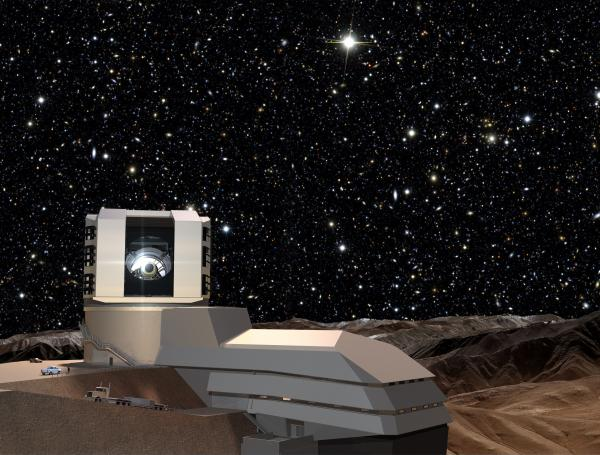
\includegraphics[width=12cm,height=7cm]{report/figures/LSST.jpg}
    \caption{Télescope LSST}
    \label{fig:modeling_shema}
\end{figure}
\newline Il sera construit en tenant compte des paramètres définis sur le tableau ci-dessous.
\newline
\begin{tabular}{|p{10cm}|p{6cm}|}
\hline 
Paramètres & Valeurs \\
\hline 
 Site & Cerro Pachón Chili 1ère \\
\hline 
 1ère lumière & 2020 \\
\hline 
 Durée de vie nominale & 10 ans\\
\hline 
 Type de télescope & Paul Baker / Mersenne Schmidt grand champ \\
\hline 
Taille du sondage & 20 000 deg2 \\
\hline 
Champ de vue & 9.62 deg2 \\
\hline 
Longueur focale & 10.2 m Diamètre \\
\hline 
Diamètre effectif & 6.5 m \\
\hline 
Étendue & 319 m2/deg2 \\
\hline 
Résolution angulaire & 0.2 seconde d'arc / pixel\\
\hline 
Nombre de filtres & 6 (u g r i z y) \\
\hline 
Spectre photométrique & 310 à 1060 nm \\
\hline 
Durée d'exposition (tvis) & 30 s (2×15 s) \\
\hline 
Nombre de jours entre chaque visite & 3 à 4 \\
\hline 
Proportion du temps pour le programme principal & 90\% \\
\hline 
Proportion du temps pour les programmes spécifiques & 10\% \\
\hline
\end{tabular}
\newline
\newline

\textbf{La camera de LSST}: Placée au centre du miroir M2, la caméra de LSST sera la plus grande caméra CCD jamais réalisée, avec un diamètre de 1.6 m, une longueur de 3 m pour un poids de 2 800 kg. En complément du plan focal de capteurs CCD, elle sera composée du correcteur de champ, d'un carrousel de 5 filtres.
\newline
\textbf{Les filtres }: Les cinq premiers des six filtres de LSST sont modélisés à partir de ceux de SDSS. La bande passante de LSST a été complétée aux grandes longueurs d'onde par l'ajout du filtre y, centré sur 1018 nm. La transmission de ces six filtres, est représentée sur la figure ci-dessous, sur laquelle nous avons également tracée la transmission de l'optique (miroirs et lentilles, en orange) ainsi que l'efficacité quantique des CCDs (en violet). Les transmissions finales des filtres tiennent compte de ces deux quantités. L'ajout du filtre supplémentaire y est motivé par la gamme de redshift accessible à LSST (les objets les plus lointains sont vus avec un spectre fortement rougi, ce qui nécessite l'utilisation d'un filtre supplémentaire) et rendu possible grâce à la grande sensibilité des capteurs CCD
\newline
\begin{figure}[!h]
    \centering
    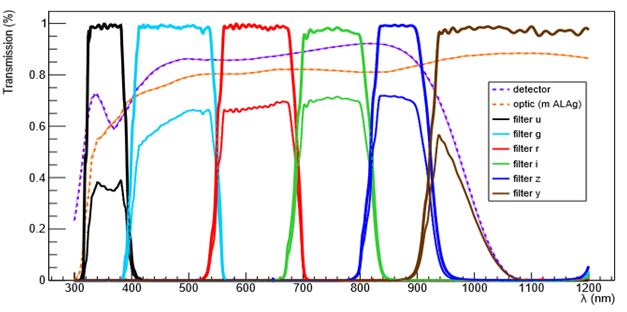
\includegraphics[width=12cm,height=7cm]{report/figures/filtre1.JPG}
    \caption{Transmission des six filtre du LSST en fonction de la longueur d'onde.}
    \label{fig:modeling_shema}
\end{figure}
\newline
Les caractéristiques de la bande passante de chacun des filtres sont résumées ci dessous.
\begin{figure}[!h]
    \centering
    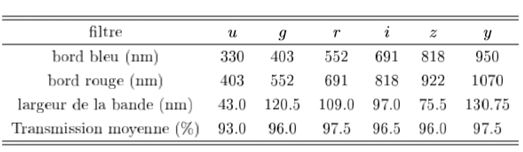
\includegraphics{report/figures/filtre2.JPG}
    \caption{Transmission des six filtre du LSST en fonction de la longueur d'onde.}
    \label{fig:modeling_shema}
\end{figure}


\subsection{La stratégie d'observation du télescope LSST}
Le principe fondamental de LSST est de balayer l'ensemble du ciel observable depuis le Chili avec un champ profond, large, et de manière rapide, avec une stratégie d'observation spécifique. Cette dernière est déterminée de façon à maximiser la qualité des observations scientifiques tout en minimisant les temps morts, avec une sélection appropriée du filtre en temps réel, et en fonction des conditions météorologiques. Bien que la stratégie d'observation ne soit pas encore complètement déterminée à ce jour, environ 90\% du temps devrait être consacré au sondage principal. Celui-ci, dit (Universal cadence), devrait conduire à la réalisation d’une base de données répondant à la plupart des objectifs de science.  Les 10\% restants seront consacrés à la réalisation de champs plus profonds, avec des temps entre deux visites très courts (∼ 1 minute), et à l'observation de régions particulières, tel que le plan de l'écliptique, le plan galactique ou les nuages de Magellan.
La cadence d'observation principale va générer un flux continu de données brutes avec une production d'environ 15 terabyte (TB) par nuit. On estime qu'après 10 ans de fonctionnement, 11 Data Release seront produites à partir d'un ensemble de données approchant 500 Pentabyte(PB) pour l'imagerie d'images et environs environ 50 PB pour les catalogues.
\subsection{Gestion de données collectées}
L'importance des volumes de données produites, l'aspect temporel des phénomènes observés et la complexité des processus traités imposent un traitement en temps réel et automatisé des données. Ainsi les données collectées par LSST seront automatiquement réduites en images et en catalogues par le système. Les données seront traitées en suivant trois niveaux :
\begin{itemize}
    \item Traitement en temps réel: archivage des images brutes générées pendant la nuit d'observation et émission des alertes (détections de nouvelles source, ou sources dont les propriétés ont changées depuis la dernière observation) dans les 60 secondes qui suivent la détection.
    \item Une fois par an, les données seront retraitées afin de fournir un catalogue et des images parfaitement calibrées (une calibration photométrique et astrométrique uniforme sur le catalogue sera fournie).
    \item Les produits de données de niveau 3 sont issu d'une combinaison des niveaux 1 et 2 afin de répondre à certaine problématiques scientifiques particulières. Le système de gestion des données (Data Management System DMS) va faciliter cette étape du traitement des données en créant des logiciels et des interfaces (API pour Application Programming Interfaces) permettant le développement des logiciels d'analyse.
\end{itemize}

L’une des principales difficultés que rencontreront les scientifiques est l’exploitation des données qui seront issues des observations.
Pour pallier à ces difficultés les concepteurs du projet LSST ont lancés le projet PLAsTiCC  Photometric LSST Astronomical Time-Series Classification Challenge) dont le but est de concevoir un modèle permettant de classer les objets observés par le télescope LSST.

\section{PLAsTiCC  (Photometric LSST Astronomical Time-Series Classification Challenge)}
Afin de faciliter l’exploitation de données collectées, LSST demande à Kaggle de l’aider à se préparer à la classification des données des nouvelles observations à travers une compétition. 
Le but de cette compétition est d’amener les concurrents  à construire un modèle de  classification qui permettra de classer  les sources  des objets astronomiques observés. 
Le modèle à construire doit tenir compte du fait que les données qui seront issues des observations astronomique ont une luminosité qui varie au cours du temps et forment une série temporelle.
Les organisateurs du challenge ont mis à la disposition des compétiteurs un jeux de données à partir duquel ils doivent construire le modèle.
Le jeux de données mis à notre disposition fera l’objet d’une étude détaillé dans la section qui suit.
\chapter{Compréhension du problème}
Étant la première tâche que nous avons réalisée, la phase de compréhension du problème est la première phase de gestion de projet de datamining. Cette première étape consiste à bien comprendre les éléments métiers et problématique que le datamining vise à résoudre ou à améliorer.
Pour mieux cerner la problématique et comprendre les objectifs à atteindre, nous allons débuter par contextualiser le problème.
\section{Contexte du problème}
Le développement de la théorie de la relativité générale couplée à de nombreuses observations astrophysiques ont permis l'élaboration d'un modèle, décrivant l'histoire de l'Univers, son évolution, son expansion et sa composition énergétique.
Les observations des galaxies et plus récemment, celles des supernovae, ont montré que notre univers est en expansion et même en expansion accélérée, ce qui ne peut se concevoir simplement compte-tenu de la force gravitationnelle qui tend à agglomérer la matière.
Du fait de l'expansion de l'Univers, les objets lointains voient leurs spectres décalés vers le rouge. La mesure de ce décalage (couramment nommé redshift) est une mesure indirecte de la distance à laquelle se trouve l'objet observé mais également une mesure du paramètre d'expansion, ce qui permet d'étudier les caractéristiques de l'énergie noire. Grâce à de nombreuses sondes observationnelles il est possible d'étudier l'évolution de l'Univers au cours du temps.
Afin d'obtenir les observations nécessaires, de nombreux projets ont vu le jour. Parmi eux, le \textbf{Large Synoptic Survey Telescope (LSST)} qui est un télescope grand champ qui devrait permettre l'observation de milliards de galaxies.
\section{Présentation du projet LSST (Large Synoptic Survey Telescope)}
Le projet LSST  est un projet international dont les objectifs de LSST balayent quatre thèmes de science à savoir :
\begin{itemize}
    \item La recherche et la compréhension de la matière noire.
    \item La recherche et la compréhension de l'énergie noire.
    \item L'étude des objets transitoires.
    \item L'étude de la Voie Lactée et du système solaire.
\end{itemize}
Chacun de ces thèmes va imposer des contraintes sur l'instrument et sa capacité d'observation.
Elles seront utilisées pour optimiser l'ensemble des paramètres caractéristiques du télescope.
\subsection{Présentation du télescope LSST}
\textbf{Le télescope LSST} est un télescope optique de grande taille en cours de construction au nord du Chili et caractérisé par un champ d’observation très large. Il observeras dans le domaine de l'optique, la totalité de l'hémisphère sud pendant plus de dix ans.
Son optique compacte sera composée de trois miroirs et une caméra avec un diamètre de 64 cm, 189 CCDs et plus de 3 milliards de pixels, sera la plus importante jamais construite. Son champ de vue à la fois large et profond va permettre l'étude de nombreux sujets scientifiques, de l'exploration intensive du système solaire aux mesures de précision des paramètres cosmologiques. 
Les mesures atmosphériques réalisées depuis 10 ans sur le site (depuis le Cerro Tololo Inter-American Observatory CTIO) montrent que plus de 80\% des nuits sont propices à l'observation avec d'excellentes conditions atmosphériques.
En plus des excellentes conditions d'observation, LSST bénéficiera d'une infrastructure (conditions d'accès ...) facilitée par la présence de télescopes d'envergure déjà en fonctionnement sur ce site. 
\newline
\newline
\begin{figure}[!h]
    \centering
    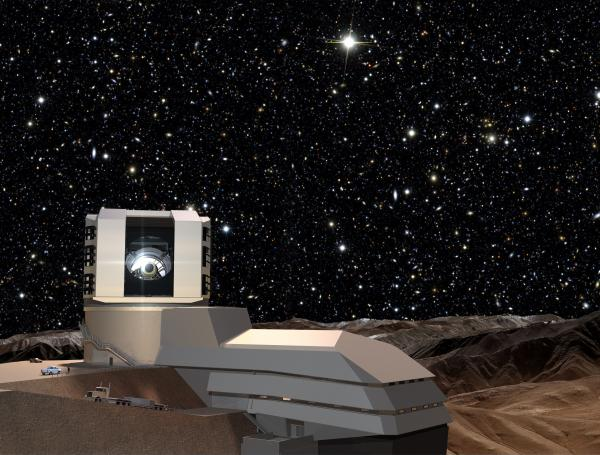
\includegraphics[width=12cm,height=7cm]{report/figures/LSST.jpg}
    \caption{Télescope LSST}
    \label{fig:modeling_shema}
\end{figure}
\newline Il sera construit en tenant compte des paramètres définis sur le tableau ci-dessous.
\newline
\begin{tabular}{|p{10cm}|p{6cm}|}
\hline 
Paramètres & Valeurs \\
\hline 
 Site & Cerro Pachón Chili 1ère \\
\hline 
 1ère lumière & 2020 \\
\hline 
 Durée de vie nominale & 10 ans\\
\hline 
 Type de télescope & Paul Baker / Mersenne Schmidt grand champ \\
\hline 
Taille du sondage & 20 000 deg2 \\
\hline 
Champ de vue & 9.62 deg2 \\
\hline 
Longueur focale & 10.2 m Diamètre \\
\hline 
Diamètre effectif & 6.5 m \\
\hline 
Étendue & 319 m2/deg2 \\
\hline 
Résolution angulaire & 0.2 seconde d'arc / pixel\\
\hline 
Nombre de filtres & 6 (u g r i z y) \\
\hline 
Spectre photométrique & 310 à 1060 nm \\
\hline 
Durée d'exposition (tvis) & 30 s (2×15 s) \\
\hline 
Nombre de jours entre chaque visite & 3 à 4 \\
\hline 
Proportion du temps pour le programme principal & 90\% \\
\hline 
Proportion du temps pour les programmes spécifiques & 10\% \\
\hline
\end{tabular}
\newline
\newline

\textbf{La camera de LSST}: Placée au centre du miroir M2, la caméra de LSST sera la plus grande caméra CCD jamais réalisée, avec un diamètre de 1.6 m, une longueur de 3 m pour un poids de 2 800 kg. En complément du plan focal de capteurs CCD, elle sera composée du correcteur de champ, d'un carrousel de 5 filtres.
\newline
\textbf{Les filtres }: Les cinq premiers des six filtres de LSST sont modélisés à partir de ceux de SDSS. La bande passante de LSST a été complétée aux grandes longueurs d'onde par l'ajout du filtre y, centré sur 1018 nm. La transmission de ces six filtres, est représentée sur la figure ci-dessous, sur laquelle nous avons également tracée la transmission de l'optique (miroirs et lentilles, en orange) ainsi que l'efficacité quantique des CCDs (en violet). Les transmissions finales des filtres tiennent compte de ces deux quantités. L'ajout du filtre supplémentaire y est motivé par la gamme de redshift accessible à LSST (les objets les plus lointains sont vus avec un spectre fortement rougi, ce qui nécessite l'utilisation d'un filtre supplémentaire) et rendu possible grâce à la grande sensibilité des capteurs CCD
\newline
\begin{figure}[!h]
    \centering
    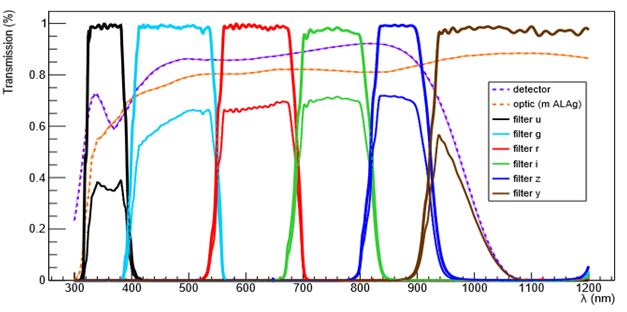
\includegraphics[width=12cm,height=7cm]{report/figures/filtre1.JPG}
    \caption{Transmission des six filtre du LSST en fonction de la longueur d'onde.}
    \label{fig:modeling_shema}
\end{figure}
\newline
Les caractéristiques de la bande passante de chacun des filtres sont résumées ci dessous.
\begin{figure}[!h]
    \centering
    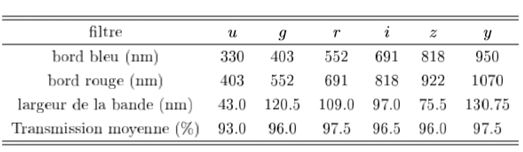
\includegraphics{report/figures/filtre2.JPG}
    \caption{Transmission des six filtre du LSST en fonction de la longueur d'onde.}
    \label{fig:modeling_shema}
\end{figure}


\subsection{La stratégie d'observation du télescope LSST}
Le principe fondamental de LSST est de balayer l'ensemble du ciel observable depuis le Chili avec un champ profond, large, et de manière rapide, avec une stratégie d'observation spécifique. Cette dernière est déterminée de façon à maximiser la qualité des observations scientifiques tout en minimisant les temps morts, avec une sélection appropriée du filtre en temps réel, et en fonction des conditions météorologiques. Bien que la stratégie d'observation ne soit pas encore complètement déterminée à ce jour, environ 90\% du temps devrait être consacré au sondage principal. Celui-ci, dit (Universal cadence), devrait conduire à la réalisation d’une base de données répondant à la plupart des objectifs de science.  Les 10\% restants seront consacrés à la réalisation de champs plus profonds, avec des temps entre deux visites très courts (∼ 1 minute), et à l'observation de régions particulières, tel que le plan de l'écliptique, le plan galactique ou les nuages de Magellan.
La cadence d'observation principale va générer un flux continu de données brutes avec une production d'environ 15 terabyte (TB) par nuit. On estime qu'après 10 ans de fonctionnement, 11 Data Release seront produites à partir d'un ensemble de données approchant 500 Pentabyte(PB) pour l'imagerie d'images et environs environ 50 PB pour les catalogues.
\subsection{Gestion de données collectées}
L'importance des volumes de données produites, l'aspect temporel des phénomènes observés et la complexité des processus traités imposent un traitement en temps réel et automatisé des données. Ainsi les données collectées par LSST seront automatiquement réduites en images et en catalogues par le système. Les données seront traitées en suivant trois niveaux :
\begin{itemize}
    \item Traitement en temps réel: archivage des images brutes générées pendant la nuit d'observation et émission des alertes (détections de nouvelles source, ou sources dont les propriétés ont changées depuis la dernière observation) dans les 60 secondes qui suivent la détection.
    \item Une fois par an, les données seront retraitées afin de fournir un catalogue et des images parfaitement calibrées (une calibration photométrique et astrométrique uniforme sur le catalogue sera fournie).
    \item Les produits de données de niveau 3 sont issu d'une combinaison des niveaux 1 et 2 afin de répondre à certaine problématiques scientifiques particulières. Le système de gestion des données (Data Management System DMS) va faciliter cette étape du traitement des données en créant des logiciels et des interfaces (API pour Application Programming Interfaces) permettant le développement des logiciels d'analyse.
\end{itemize}

L’une des principales difficultés que rencontreront les scientifiques est l’exploitation des données qui seront issues des observations.
Pour pallier à ces difficultés les concepteurs du projet LSST ont lancés le projet PLAsTiCC  Photometric LSST Astronomical Time-Series Classification Challenge) dont le but est de concevoir un modèle permettant de classer les objets observés par le télescope LSST.

\section{PLAsTiCC  (Photometric LSST Astronomical Time-Series Classification Challenge)}
Afin de faciliter l’exploitation de données collectées, LSST demande à Kaggle de l’aider à se préparer à la classification des données des nouvelles observations à travers une compétition. 
Le but de cette compétition est d’amener les concurrents  à construire un modèle de  classification qui permettra de classer  les sources  des objets astronomiques observés. 
Le modèle à construire doit tenir compte du fait que les données qui seront issues des observations astronomique ont une luminosité qui varie au cours du temps et forment une série temporelle.
Les organisateurs du challenge ont mis à la disposition des compétiteurs un jeux de données à partir duquel ils doivent construire le modèle.
Le jeux de données mis à notre disposition fera l’objet d’une étude détaillé dans la section qui suit.